\section*{Consigna}

Se tiene la siguiente topología con sus datos:

\begin{figure}[H]
    \centering
    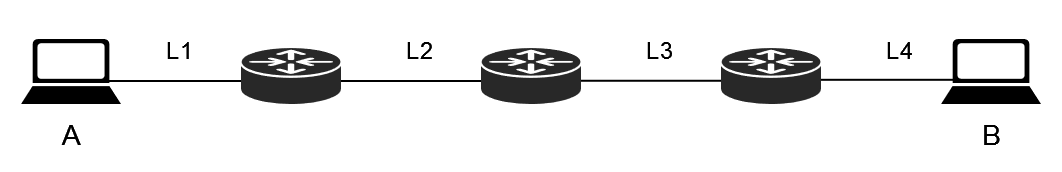
\includegraphics[width=0.9\linewidth]{Images/topologia.png}
\end{figure}

\vspace{-5mm}
{
\renewcommand{\arraystretch}{1.5}
\begin{table}[H]
    \centering
    \begin{tabular}{|c|c|c|c|c|}
    \hline
     & L1 & L2 & L3 & L4 \\ \hline
    Distancia & 100 m & 10 km & 4 km & 100 m \\ \hline
    Ancho de banda & 10 Mbps & 200 Mbps & 200 Mbps & 10 Mbps \\ \hline
    Velocidad del medio & $1,7\cdot 10^5$ km/s & $2\cdot 10^5$ km/s & $2\cdot 10^5$ km/s & $1,7\cdot 10^5$ km/s  \\ \hline
    \end{tabular}
\end{table}
}



\begin{enumerate}
    \item Calcular el RTT entre \textbf{A} y \textbf{B} (despreciar tiempo de encolado).
    \item Calcular el tiempo necesario para enviar un paquete de 1000B desde \textbf{A} hacia \textbf{B}.
\end{enumerate}

\section*{Resolución}

\noindent
\textbf{1)}\tab Primero hay que entender qué es el RTT. James Kurose dice ``we define the round-trip time (RTT), which is the time it takes for a small packet to travel from client to server and then back to the client. The RTT includes packet-propagation delays, packet-queuing delays in intermediate routers and switches, and packet-processing delays.''

Siendo que es el tiempo que tarda un paquete pequeño en ir ida y vuelta desde el cliente es:

\vspace{0.5\baselineskip}
\hfil
{\large
$\text{RTT} =
2 \cdot \left(t_{\text{prop}} + t_{\text{queue}} + t_{\text{proc}} \right)$
}
\hfil

{
\noindent\large
\underline{$t_{\text{prop}}$:}
}

\skipline
Para calcular el tiempo de propagación entre el cliente y el servidor habrá que calcular el tiempo de propagación para cada enlace:

$$t_{\text{prop}} = \dfrac{\text{Distancia}}{\text{V del medio}}$$

$t_{\text{prop-1}} =
\dfrac{0,1\text{ km}}{1,7\cdot 10^5\text{ km}/\text{s}} =
5,88 \cdot 10^{-7}\text{ s} = 588\text{ns}$

\vspace{0.5\baselineskip}
$t_{\text{prop-2}} =
\dfrac{10\text{ km}}{2\cdot 10^5\text{ km}/\text{s}} =
5 \cdot 10^{-5}\text{ s} = 50\mu\text{s}$

\vspace{0.5\baselineskip}
$t_{\text{prop-3}} =
\dfrac{4\text{ km}}{2\cdot 10^5\text{ km}/\text{s}} =
2 \cdot 10^{-5}\text{ s} = 20\mu\text{s}$

\vspace{0.5\baselineskip}
$t_{\text{prop-4}} = t_{\text{prop-1}} = 588\text{ns}$ (Los enlaces son iguales)

\vspace{\baselineskip}
$t_{\text{prop}} =
t_{\text{prop-1}} + t_{\text{prop-2}} + t_{\text{prop-3}}+ t_{\text{prop-4}} = 71,2 \mu\text{s}$


\skipline
{
\noindent\large
\underline{$t_{\text{queue}}$:}
}

\skipline
En un escenario real el tiempo de encolado es variable, se lo podría llegar a estimar o tomar un promedio. En este ejercicio se lo desprecia.


\skipline
{
\noindent\large
\underline{$t_{\text{proc}}$:}
}

\skipline
El $t_{\text{proc}}$ suele ser del orden de los ns. Analizando el valor del tiempo de propagación ya obtenido puede despreciarse.

\skipline
\noindent
\underline{Finalmente:}

\hfil
\fbox{
$\text{RTT} =
2 \cdot \left(t_{\text{prop}} + \xcancel{t_{\text{queue}}} + \xcancel{t_{\text{proc}}} \right)=
2 \cdot 71,2 \mu\text{s} =
142,4 \mu\text{s}
$}
\hfil



\skipline
\noindent
\textbf{2)}\tab El tiempo necesario para enviar un paquete desde \textbf{A} hacia \textbf{B} será:

\vspace{0.5\baselineskip}
\hfil
{\large
$T =
t_{\text{prop}} + t_{\text{queue}} + t_{\text{proc}} + t_{\text{trans}}$
}
\hfil

\vspace{0.5\baselineskip}
Ya se hizo el análisis de todos los $t$ excepto por el de transmisión.


\skipline
{
\noindent\large
\underline{$t_{\text{trans}}$:}
}
$$t_{\text{trans}} = \dfrac{\text{Tamaño del paquete}}{\text{Ancho de banda}}$$

$t_{\text{trans-1}} =
\dfrac{8.000\text{b}}{10 \cdot 2^{20} \text{b}/\text{s}} =
7,63\cdot 10^{-4} \text{s} =
763 \mu\text{s}
$

\vspace{0.5\baselineskip}
$t_{\text{trans-2}} =
\dfrac{8.000\text{b}}{200 \cdot 2^{20} \text{b}/\text{s}} =
3,81\cdot 10^{-5} \text{s} =
38,1 \mu\text{s}
$

\vspace{0.5\baselineskip}
$t_{\text{trans-3}} =
t_{\text{trans-2}} =
38,1 \mu\text{s}
$

\vspace{0.5\baselineskip}
$t_{\text{trans-4}} =
t_{\text{trans-1}} =
763 \mu\text{s}
$

\vspace{\baselineskip}
$t_{\text{trans}} =
t_{\text{trans-1}} + t_{\text{trans-2}} + t_{\text{trans-3}} + t_{\text{trans-4}} = 1,60 \text{ms}
$

\skipline
\noindent
\underline{Finalmente:}

\vspace{0.5\baselineskip}
\hfil
{\large
\fbox{
$T =
t_{\text{prop}} + \xcancel{t_{\text{queue}}} + \xcancel{t_{\text{proc}}} + t_{\text{trans}} = 71,2 \mu\text{s} + 1,60 \text{ms} =
1,67 \text{ms}$
}
}
\hfil